\documentclass[10pt,twocolumn,letterpaper]{article}
\usepackage[T1]{fontenc}
\usepackage[pagenumbers]{cvpr}
\usepackage{times,graphicx,amsmath,amssymb,booktabs,multirow}
\usepackage{tikz}
\usetikzlibrary{arrows.meta,positioning}
\definecolor{cvprblue}{rgb}{0.21,0.49,0.74}
\usepackage[breaklinks,colorlinks,allcolors=cvprblue]{hyperref}
\def\confName{AIAA3201}
\def\confYear{2027}
\captionsetup{hypcap=false}
\setlength{\tabcolsep}{5pt}
\newcommand{\panel}[3]{\begin{figure}[tb]\centering\includegraphics[width=#2\linewidth]{images/#1}\caption{#3}\end{figure}}
\newcommand{\widepage}[3]{\begin{figure*}[t]\centering\includegraphics[width=#2\textwidth]{images/#1}\caption{#3}\end{figure*}}
\title{Geometry, Metric Depth, and Temporal Fusion:\\A Controlled Small-Model Study}
\author{Qinchuan XIAO \qquad Jun Yu Eugene YIP\\
HKUST (Guangzhou)\\
AIAA3201 Project 3 --- Spring 2027 specification}
\begin{document}
\maketitle
\begin{abstract}
We evaluate calibrated stereo, pretrained monocular metric depth, and relative video depth under explicitly separated protocols. StereoSGBM on 15 Middlebury trainQ scenes yields 1.311 px mean scene-level disparity MAE at 62.65\% pooled coverage after an extra left--right check; lower conditional error comes with substantial rejection. RGB-only UniDepthV2 ViT-S obtains 0.1108 AbsRel, 0.3928 m RMSE, and 0.8948 $\delta_1$ on all 654 NYUv2 test images under the course protocol. On the supplied rollercoaster clip, Video Depth Anything reduces an observed frame-wise color fluctuation, while fine structures remain incomplete. We implement causal flow-guided fusion and control its alignment, rejection, confidence, history source, and strength. More aggressive smoothing lowers a temporal diagnostic but can introduce ghosts; confidence weighting retains current-frame contours while leaving residual fluctuations. Streaming reduces measured peak GPU memory by about 71\% but shows startup variation. One targeted confidence relaxation gives small diagnostic gains without clear visual benefit. Background blur improves mainly through its thresholds. All results are from saved, verified outputs; supplementary comparisons are post-hoc, not new blind tests. Code: \url{https://github.com/Lingxiaolingqc/MMDEVC/}.
\end{abstract}

\section{Introduction}
A plausible depth map can have wrong scale, missing fine structure, or temporal variation. Calibrated stereo measures disparity; monocular metric models infer scale from learned priors; relative video models need not return metres. We evaluate these failures separately.

This study follows the course sequence: geometry and frame-wise baselines, a metric model and a video model, one lightweight improvement, then an application. We choose flow-guided fusion, operating on unchanged Depth Anything V2 (DA) outputs. We also compare official streaming VDA and one bounded confidence refinement. No foundation-model training, test-GT scale fitting, or metric-video route is added. Static NYUv2 provides depth accuracy; unannotated videos provide visual and temporal diagnostics.

We report coverage and negative results alongside conditional errors. Stable maps may accumulate stale structures; better-looking blur may reflect application thresholds rather than better depth.

\section{Related Work}
SGM aggregates stereo matching costs along multiple paths~\cite{sgm}. OpenCV StereoSGBM is a modified implementation~\cite{opencv}, not an exact reproduction of every original component. Middlebury provides calibrated stereo scenes~\cite{middlebury}; KITTI established important driving-scene benchmarks~\cite{kitti}, but is not evaluated here.

DPT reassembles transformer features for dense prediction~\cite{dpt}. Depth Anything scales unlabeled supervision~\cite{dav1}; DA V2 combines synthetic teaching with pseudo-labeled real images~\cite{dav2}. We use its Small relative release.

UniDepth conditions metric prediction on a learned camera representation~\cite{unidepth}; UniDepthV2 adds edge-oriented training and uncertainty~\cite{unidepthv2}. We use RGB-only Z depth without GT intrinsics. Depth Pro offers multiscale inference and sharp-boundary training~\cite{depthpro}, but is not evaluated.

RAFT uses all-pairs correlations and recurrent flow refinement~\cite{raft}. Our lightweight route instead uses Farneb\"ack flow~\cite{farneback}. Video Depth Anything (VDA) replaces the DA V2 head with a spatial-temporal head and supports keyframe-based long-video inference~\cite{vda}. It is an independent pretrained reference, not a component of our fusion.

\begin{center}\begin{minipage}{\linewidth}\centering
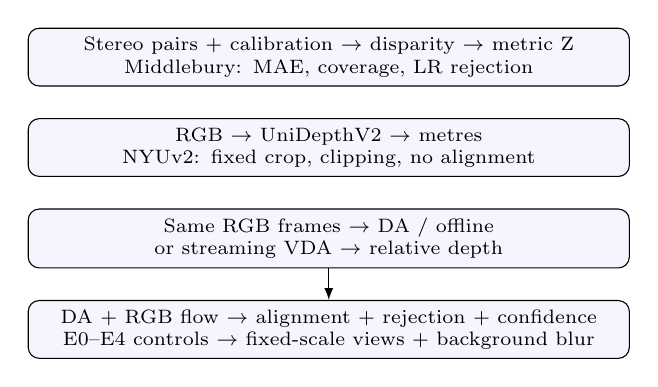
\begin{tikzpicture}[node distance=4mm, every node/.style={font=\scriptsize,align=center},
box/.style={draw,rounded corners,fill=blue!4,text width=7.4cm,minimum height=5mm},
arr/.style={-{Latex[length=1.5mm]}}]
\node[box] (s) {Stereo pairs + calibration $\rightarrow$ disparity $\rightarrow$ metric Z\\Middlebury: MAE, coverage, LR rejection};
\node[box,below=of s] (n) {RGB $\rightarrow$ UniDepthV2 $\rightarrow$ metres\\NYUv2: fixed crop, clipping, no alignment};
\node[box,below=of n] (v) {Same RGB frames $\rightarrow$ DA / offline or streaming VDA $\rightarrow$ relative depth};
\node[box,below=of v] (f) {DA + RGB flow $\rightarrow$ alignment + rejection + confidence\\E0--E4 controls $\rightarrow$ fixed-scale views + background blur};
\draw[arr] (v)--(f);
\end{tikzpicture}
\captionof{figure}{Three evaluation branches. Stereo and NYU have GT; the video branch has no depth GT. Only DA is modified by fusion.}
\end{minipage}\end{center}

\section{Methods and Evaluation}
\subsection{Stereo geometry and validity}
We run OpenCV 4.13 StereoSGBM on the 15 quarter-resolution Middlebury training pairs. Development uses Adirondack and Pipes; the other 13 scenes are separated from parameter selection. The all-15 summary is descriptive, not an official hidden-test score. Settings include a $3\times3$ block, uniqueness ratio 10, speckle window 100, speckle range 2, and prefilter cap 31. Search ranges follow the scene calibration.

The left disparity is $d=x_L-x_R$. OpenCV's signed fixed-point output is divided by 16. With quarter-resolution focal length $f$, baseline $B$ in millimetres, and calibration offset $c=\mathrm{doffs}$,
\begin{equation}
Z(d)=\frac{fB}{1000(d+c)}.
\label{eq:depth}
\end{equation}
Invalid matcher values, nonfinite outputs, and nonpositive Z are excluded from conditional errors. The optional extra left--right (LR) check samples the reverse match at the left correspondence and requires an in-bounds valid sample and residual at most 1 px. LR off/on retains the same original matching and OpenCV internal settings; it changes a mask, not retained disparities.

All-GT evaluation uses finite, positive GT disparities. We also report the supplied nonoccluded region. Coverage divides valid predictions by the fixed GT count. Disparity MAE and Z RMSE are conditional on valid predictions, whereas the supplementary bad-$1$ fraction counts invalid predictions as failures. Scene-level errors are macro averaged; coverage and bad-$1$ are pixel pooled.

\subsection{Pretrained metric and relative models}
UniDepthV2 ViT-S uses the official RGB-only \texttt{infer} path with predicted intrinsics and resolution level 0. Outputs are restored to $480\times640$. The official NYUv2 split~\cite{nyu} contains 795 training and 654 test images; three training-side examples were used for development checks. No model is locally trained. Upstream pretraining overlap is not independently audited.

NYU evaluation uses filled GT depths in metres, Python crop \texttt{[45:471,41:601]}, GT range $[0.001,10]$ m, and predictions clipped to that range. For each image's GT domain $\Omega$:
\begin{align}
\mathrm{AbsRel}&=\frac{1}{|\Omega|}\sum_{\Omega}\frac{|p-g|}{g},\\
\mathrm{RMSE}&=\sqrt{\frac{1}{|\Omega|}\sum_{\Omega}(p-g)^2},\\
\delta_1&=\frac{1}{|\Omega|}\sum_{\Omega}
\mathbf{1}\!\left[\max(p/g,g/p)<1.25\right].
\end{align}
Each metric is averaged equally over 654 images. No test scale or shift is fitted. These are course-protocol results, not claimed paper-score reproductions.

DA V2 Small processes frames independently; VDA Small uses official offline inference. Both use FP16, requested input size 364, and restored $640\times360$ outputs. The actual encoder spatial size is $364\times644$. The pinned repository clip contains 70 frames at 24 fps, not the requested 100. We process all 70 original frames without duplication and disclose this discrepancy; the user accepted this handling, which is not teacher approval. Tokyo, an optional repository example, supplies 100 frames at 15 fps for development. No self-recorded data are required.

\subsection{Causal flow-guided fusion}
Let $D_t$ be current DA and $H_{t-1}$ previous raw or fused depth. Backward flow warps history into current coordinates:
\begin{equation}
\widehat D_t=(1-w_t)D_t+w_t\,W(H_{t-1}).
\end{equation}
E0 returns DA. E1 blends at identical coordinates. E2 adds flow warping. E3 rejects out-of-bounds, photometrically inconsistent, and forward--backward (FB) inconsistent samples. E4 adds continuous confidence:
\begin{equation}
w_t=\alpha M_t\exp\!\left[-\frac{r_p}{.1}-\frac{r_f}{1}
-\frac{r_d}{.1}-\frac{r_e}{.1}\right].
\label{eq:confidence}
\end{equation}
Here $r_p$ is RGB residual, $r_f$ is FB residual in pixels, $r_d$ is absolute depth disagreement, and $r_e$ is a four-neighbor edge magnitude; the last two are divided by the current DA frame's P1--P99 span. This span only affects confidence, never raw predictions or per-frame display scaling. The hard gate requires $r_p\le.2$ and $r_f^2\le.01(\|F_b\|^2+\|W(F_f)\|^2)+.5$. These are heuristic weights, not calibrated probabilities.

Farneb\"ack uses pyramid scale .5, three levels, window 15, three iterations, polynomial neighborhood 5 and sigma 1.2. The frozen maximum weight is $\alpha=.70$. Recursive history uses $\widehat D_{t-1}$; pairwise uses $D_{t-1}$. First-frame outputs equal DA.

\subsection{Diagnostics and evidence boundaries}
Video colors use one fixed whole-clip P1--P99 range per model. E0--E4 share DA's range; VDA has its own. Relative zero values are valid finite outputs, not zero metres.

For common RGB/flow reference pixels, $T$ averages $\min(|D_t-W(D_{t-1})|/s,1)$ with fixed clip span $s$. Invalid pairs pay 1; valid-pair coverage is also reported. Departure measures mean $|\widehat D-D|/s$. Neither quantity is GT accuracy or a perceptual score. Real motion, flow error, and smoothing affect them. We inspected matched stills and consecutive contact sheets, with frame indices and ROI coordinates recorded; this is not full real-time playback. Test footage had been viewed before the renewed freeze, and supplementary analyses are post-hoc.

\widepage{jadeplant.png}{1}{Jadeplant diagnostic from unchanged StereoSGBM outputs. Gray denotes invalid or unavailable values. GT and prediction share display ranges; the last panel shows pre-rejection LR residual. The image-wide validity title differs from GT-domain coverage. Display clipping does not clip evaluation values.}
\section{Part 1: Stereo and Frame-Wise Baselines}
\subsection{LR reliability versus coverage}
Table~\ref{tab:stereo} shows that the optional custom LR check reduces conditional error but rejects many pixels. It cannot be described as correcting disparities. Across all-GT regions, 595,472 previously valid predictions are removed. Only 32.56\% of those exceed 1 px GT error; 67.44\% are within 1 px. Moreover, 82.20\% of rejections have no comparable right match. Lack of a reverse match is not proof that the left disparity was wrong.

\begin{center}\begin{minipage}{\linewidth}\centering
\captionof{table}{15-scene descriptive summary. Errors are scene macro averages on valid predictions; coverage and bad-$1$ are pooled over fixed GT pixels.}
\label{tab:stereo}
\small
\begin{tabular}{llrrrr}
\toprule
GT & LR & MAE px & Cov.\% & Z RMSE m & Bad-$1$\%\\
\midrule
All & off & 1.839 &75.63&.202&35.97\\
All & on &1.311&62.65&.150&44.73\\
Nonocc. &off&1.426&82.33&.169&28.05\\
Nonocc. &on&1.019&68.84&.122&37.82\\
\bottomrule
\end{tabular}
\end{minipage}\end{center}

On the 13 evaluation scenes, LR-on MAE is 1.337 px at 61.26\% coverage. The all-15 number includes development, so it should not replace this subset when discussing separation from tuning. 

\subsection{Structure, tails, and metric conversion}
The eight-panel Jadeplant view reveals fragmented fine branches and clutter boundaries while preserving larger surfaces. Its conditional MAE is 3.524 px and GT-domain coverage 37.39\%; its P95 disparity error reaches 31.77 px. PianoL has 4.067 px MAE at 39.42\% coverage. A comparatively strong case, Teddy, has 0.414 px MAE and 72.96\% coverage. Figure~\ref{fig:boxes} shows why a mean alone is insufficient.

\panel{stereo_boxes.png}{1}{Selected scenes after LR: exact valid-pixel quantiles, quartile boxes, median lines and P5--P95 whiskers. Labels report GT-domain coverage. Disparity and depth have separate units; omitted tails remain in the evidence CSVs.\label{fig:boxes}}

Depth error follows an exact relation, with $K=fB/1000$:
\begin{equation}
Z(d)-Z(d^*)=\frac{-K(d-d^*)}{(d+c)(d^*+c)}.
\end{equation}
We verify this to floating-point precision; it is a correctness check, not a second method. Larger Z errors can arise despite moderate disparity errors. Pipes has 0.591 m Z RMSE and GT depths up to 8.566 m. All pixels beyond 6 m belong to development Pipes, so pooled distance trends confound scene and calibration with distance. 

\widepage{nyu_cases.png}{1}{Two actual NYUv2 test cases, with matching GT/prediction scales within each row. Top: bookstore image 0088, the largest course AbsRel. Bottom: image 0033, where a modest depth RMSE coexists with missing thresholded monitor boundaries. Error is shown only inside the fixed course GT domain, capped at 2 m (top) and 0.5 m (bottom) for display; row-specific depth scales are labeled.}
\section{Part 2: Monocular Metric Depth}
\subsection{Course accuracy and protocol effects}
UniDepthV2 predicts finite positive depths over all 156,018,240 evaluated GT pixels. Table~\ref{tab:nyu} separates the required clipped protocol from an unclipped diagnostic on the same arrays. Upper clipping affects 554,689 pixels (0.3555\%) across 26 images; no lower clipping occurs. The 5.72\% RMSE decrease is a protocol effect, not a learned improvement.

\begin{center}\begin{minipage}{\linewidth}\centering
\captionof{table}{654-image equal-weight means; no alignment. The clipped row is the formal course result.}
\label{tab:nyu}
\begin{tabular}{lrrr}
\toprule
Preparation & AbsRel & RMSE m & $\delta_1$\\
\midrule
Unclipped diagnostic &.11224&.41666&.89311\\
Course-clipped &\textbf{.11078}&\textbf{.39282}&\textbf{.89478}\\
\bottomrule
\end{tabular}
\end{minipage}\end{center}

Pixel-pooled RMSE is 0.48305 m; the formal image-macro value is 0.39282 m. These aggregate square roots differently.


Median image AbsRel is 0.09455, while its P95 is 0.23950. RMSE has median 0.30862 m, P95 0.94119 m, and maximum 2.01190 m. A single average therefore understates difficult scenes.

\subsection{Scale and boundary errors}
The median across per-image median prediction/GT ratios is 1.0370; the 5th--95th percentile interval is 0.8593--1.1965. These ratios diagnose bias and are never used to fit the test predictions. Image 0088 overestimates much of the bookstore, with median ratio 1.6812 and course AbsRel 0.6198. Living-room 1208 underestimates depth (median ratio 0.6757).

Pooled RMSE by GT distance rises from 0.287 m at 1--2 m to 1.496 m at 6--10 m; the latter contains only 3.08\% of evaluated pixels. Nearer than 1 m, AbsRel is relatively high at 0.258. These groups mix objects and scenes and are not a distance-only experiment.

Our optional boundary diagnostic marks four-neighbor log-depth jumps above $\log(1.1)$, uses a 3-by-3 eroded GT domain, and allows 2 px matching tolerance. Pooled precision/recall/F1 are 0.758/0.400/0.523; macro F1 is 0.457. Prediction edges (1,290,091 pixels) are fewer than GT edges (2,295,868). These thresholds define a project diagnostic, not a published benchmark replication.

Image 0033 has RMSE 0.1475 m but boundary F1 zero: the broad room/monitor structure is present while the selected depth discontinuities are too smooth. Mirror-region discrepancies in 1293 and 1354 require caution because filled sensor GT does not independently certify the physical depth of reflections. Thirteen diagnostic images were inspected.

\widepage{video.png}{1}{Identical rollercoaster ROI at frames 14--16. DA changes bright--dark--bright over the train and nearby track. E4 leaves much of that change; VDA is more stable in this window. Passenger/seat gaps remain merged. All outputs are relative; VDA's colors use a different fixed whole-clip range, not shared metres.}
\section{Video Baselines and Fusion Results}
\subsection{Frame-wise DA versus offline VDA}
DA recovers recognizable tracks, coarse supports, and separation from the sky. The inspected large supports do not all vanish or flicker; the more precise failure is incomplete fine structure and a localized train/track color fluctuation. VDA reduces the latter at frames 14--19 but still merges small passenger and seat details. Late frames 64--69 retain jagged or filled gaps. Timing for the separate streaming comparison is defined below.

The official offline implementation uses 32-frame inputs, a 22-frame step, keyframe reuse and eight-frame overlap interpolation. The 70-frame clip is processed in four windows with final-frame padding, then truncated back to 70 outputs. The first ten input positions reuse selected earlier keyframes; this is not simply four disjoint batches. Two inspected interpolation regions, frames 24--31 and 46--53, show no prominent color seam. These observations do not establish consistency over arbitrarily long video.

\begin{center}\begin{minipage}{\linewidth}\centering
\captionof{table}{Recorded model inference, excluding loading, I/O, evaluation and rendering. GPU peak is PyTorch allocated memory; reserved memory is given in text.}
\label{tab:resources}
\small
\begin{tabular}{lrrr}
\toprule
Model & ms/output & FPS & Peak MiB\\
\midrule
DA V2 Small &36.697&27.250&268.98\\
VDA Small offline &74.235&13.471&2386.35\\
UniDepthV2 ViT-S &47.897&20.878&401.95\\
\bottomrule
\end{tabular}
\end{minipage}\end{center}

Hardware is an RTX 4060 Laptop GPU (8 GB), Windows 11, PyTorch 2.10.0+cu128, CUDA 12.8 and FP16. Reserved peaks are 304, 3164 and 456 MiB respectively. UniDepth uses encoder size $434\times574$, batch one; DA uses $364\times644$, batch one; VDA uses 32-frame windows at that spatial size. VDA ms/output divides clip-total inference time by output frames; FPS is its reciprocal, not causal latency. Stereo is CPU-only: the current Adirondack run takes 0.104 s for one measured pair after one warmup at $718\times496$, which is not a benchmark.


\subsection{Optional offline versus streaming VDA}
The official streaming API caches temporal features and accepts one RGB frame per call. We use the same Small weights, input size, precision and restored grids. Each mode has three synchronized repetitions after warmup, with cached history reset and allocator cache cleared before each sequence. The offline warmup uses a 32-frame prefix with official padding. Input RGB is already resident; loading, decoding, file I/O and rendering are excluded.

\begin{center}\begin{minipage}{\linewidth}\centering
\captionof{table}{New repeated VDA measurements: median first API return, amortized ms/output, maximum allocated MiB, and $T$ under each mode's own clip span. Tky=Tokyo; RC=rollercoaster.}
\label{tab:streaming}
\scriptsize
\begin{tabular}{llrrrr}
\toprule
Clip&Mode&First ms&ms/out&MiB&$T$\\
\midrule
Tky&Offline&9584.7&95.85&2386.4&.002941\\
Tky&Stream&69.1&57.34&685.3&.003580\\
RC&Offline&5928.5&84.69&2386.4&.011590\\
RC&Stream&91.5&62.97&682.8&.012769\\
\bottomrule
\end{tabular}
\end{minipage}\end{center}

Offline returns the whole clip; its first API return is not an intrinsic first-frame latency. Streaming subsequent-call median/P95 is 56.47/60.21 ms on Tokyo and 60.48/70.62 ms on rollercoaster. The latter exceeds the 41.67 ms budget for 24 fps. Reserved peaks are 3178 MiB offline and 806 MiB streaming. Mode blocks were sequential rather than randomized; three repeats are not three independent videos. Earlier single-run times are kept separate.

Saved offline predictions exactly match the prior run. Streaming repeats and reset-prefix replay agree exactly. Allocated memory falls about 71\%, while $T$ rises 21.71\% on Tokyo and 10.17\% on rollercoaster. Different own-span normalization and no video GT preclude an accuracy interpretation. Six uniform frames and four consecutive windows per clip show similar broad structures, but streaming startup colors vary more. Passenger gaps remain merged; no clear new broad ghosts appear in inspected motion windows. These short clips do not establish long-stream stability.

\panel{streaming.png}{1}{Rollercoaster frames 0 and 2: streaming has a darker initial train prediction before shifting toward green; offline changes less. Each mode keeps its own full-clip color range. This is an offline display, not online scale estimation.}

\subsection{E0--E4 main comparison}
\begin{center}\begin{minipage}{\linewidth}\centering
\captionof{table}{Same DA scale and public reference pixels within each clip. $D$ is departure from current DA, not GT error. All reference-pair coverages equal 1.}
\label{tab:main}
\small
\begin{tabular}{lrrrr}
\toprule
&\multicolumn{2}{c}{Tokyo}&\multicolumn{2}{c}{Rollercoaster}\\
Method &$T$&$D$&$T$&$D$\\
\midrule
E0&.005168&0&.014708&0\\
E1&.002950&.005868&.015586&.092337\\
E2&.002647&.006097&.004983&.011845\\
E3&.002609&.005916&.004653&.009546\\
E4&.003439&.002817&.012364&.001561\\
\bottomrule
\end{tabular}
\end{minipage}\end{center}

On rollercoaster, E1 worsens $T$ and creates broad support ghosts. E2 alignment markedly reduces those ghosts; E3 further limits inappropriate history but can yield mottled train interiors. E4 retains clearer current-frame contours yet smooths less. Its $T$ is 15.93\% below DA, but it is not the lowest-$T$ variant. Tokyo shows the same contour-versus-smoothing tradeoff, while E1's lower $T$ there illustrates that a small diagnostic value can coexist with bad outlines.

Reference pixels cover 89.20\% of rollercoaster and 98.17\% of Tokyo adjacent-pair pixels, excluding some difficult flow/occlusion regions. E4's estimated rollercoaster pipeline speed is 6.534 FPS from separate recorded DA (2.569 s), flow (6.628 s), and fusion (1.517 s) stages. This is a sum, not a repeated end-to-end measurement. VDA has $T=.011590$ under its own span; raw units differ, so it is not a common-unit accuracy ranking.

\widepage{modules.png}{1}{Module comparison at rollercoaster frames 15 and 35. E1 accumulates repeated supports. Flow alignment in E2 limits this spread; E3 rejects more history but produces localized mottling. E4 resembles the current DA silhouette more closely. All four share DA's fixed scale.}
\section{Controlled Supplementary Experiments}
\subsection{History source: pairwise versus recursive}
For each E1--E4 variant, only the history source changes. Pairwise uses the preceding raw prediction and still uses history; E0 is the actual no-history control. Inputs, optical flow, thresholds and weight formula remain fixed. E4's numeric weights can change because its depth-confidence term depends on history.

\begin{center}\begin{minipage}{\linewidth}\centering
\captionof{table}{Recursive reduction in $T$ relative to pairwise. Lower $T$ alone does not establish better shape or motion response.}
\small
\begin{tabular}{lrrrr}
\toprule
Clip &E1&E2&E3&E4\\
\midrule
Tokyo &30.77\%&35.84\%&36.09\%&15.28\%\\
Rollercoaster &7.84\%&44.22\%&45.23\%&0.95\%\\
\bottomrule
\end{tabular}
\end{minipage}\end{center}

Recursive E1 makes wider repeated contours than pairwise. E2 recursive leaves softer passenger contours in the inspected rollercoaster window; both E3 histories remain locally mottled. E4's pairwise/recursive images are nearly indistinguishable there. E4 changes $T$ only from .0124824 to .0123643; changing history also changes its confidence weights.


\subsection{Four soft-confidence removals}
We remove one term at a time from Eq.~\ref{eq:confidence}, retaining all hard gates and the same recursive history rule. This identifies marginal effects conditional on the other components; it is not a full interaction study.

\begin{center}\begin{minipage}{\linewidth}\centering
\captionof{table}{Leave-one-out E4 on each clip. $T$ decreases for every removal, while departure from DA increases.}
\small
\begin{tabular}{lrrrr}
\toprule
&\multicolumn{2}{c}{Tokyo}&\multicolumn{2}{c}{Rollercoaster}\\
Setting &$T$&$D$&$T$&$D$\\
\midrule
Full&.003439&.002817&.012364&.001561\\
No photo&.003200&.003433&.011977&.001843\\
No flow&.003354&.003013&.012113&.001749\\
No depth&.003243&.003523&.010948&.002569\\
No edge&.003330&.003067&.011028&.002719\\
\bottomrule
\end{tabular}
\end{minipage}\end{center}

Photo has the largest $T$ effect on Tokyo; depth and edge have larger effects on rollercoaster. Full E4 and each removal look very similar in the inspected contact sheets. We do not claim that each term visibly improves quality. Their measured role is to constrain temporal smoothing, and results depend on the clip.

\subsection{Development fusion strength}
With all other settings fixed, Tokyo $\alpha=.50/.70/.85$ yields $T=.003899/.003439/.003101$ and departure $.001844/.002817/.003741$. Increasing history reduces $T$ while changing current DA more. Matched pedestrian windows 28--33 and 60--65 reveal only subtle differences, with no clear additional harm from .85. The retained .70 setting is a conservative existing choice, not a demonstrated optimum. Test results were not used to retune it. Correlated frames do not supply independent trials, and none of these post-hoc controls is presented as a new blind test.


\subsection{One targeted refinement attempt}
We hypothesized that depth disagreement suppresses useful history in reliable interiors. Before generating candidates, we fixed one relaxation: double the depth sigma from .1 to .2, either globally (G) or selectively (S). S requires RGB residual $\le .05$, FB residual $\le .5$ px, and exclusion from a two-pixel-dilated band of normalized DA edges above .02. These masks use current raw DA and RGB flow only. All hard gates, other confidence terms and $\alpha$ stay unchanged. Each mode has its own recursive history; outside the guard, S preserves the original rule, not necessarily identical sequence values.

The dev diagnosis weakens the hypothesis: reliable-interior mean depth exponent is .0590 versus photo .1032, and mean history weight is already .5579. Only .00717\% of that region has depth exponent above one. G/S lower dev $T$ by 2.59/1.95\%, but matched pedestrian windows 28--33 and 73--78 reveal no clear visual gain. We freeze retention of original E4 before applying the unchanged candidates to the already-viewed course clip.

\begin{center}\begin{minipage}{\linewidth}\centering
\captionof{table}{Bounded refinement. CPU fusion seconds are medians of three repeats in rotated mode order; no model, flow, I/O or rendering time is included.}
\label{tab:refinement}
\small
\begin{tabular}{lrrrr}
\toprule
&\multicolumn{2}{c}{Tokyo}&\multicolumn{2}{c}{Rollercoaster}\\
Method&$T$&seconds&$T$&seconds\\
\midrule
Original&.003439&3.412&.012364&2.166\\
Global&.003350&3.001&.011767&2.504\\
Selective&.003372&7.630&.012204&5.877\\
\bottomrule
\end{tabular}
\end{minipage}\end{center}

On rollercoaster G/S reduce $T$ by 4.83/1.29\%, without clearly resolving the frame 14--16 color change or merged passenger gaps. S changes the edge band less than G (normalized mean difference from E4 .000015 versus .001031), which measures preservation, not correctness. S computes two fusion paths and a guard; its added CPU cost is implementation-specific. We keep the negative result and stop tuning.

Regional diagnosis exposes an averaging trap: reliable interiors cover 58.70\% of pixels but many have zero relative output in sky. Their positive-output subset is only 4.90\% of all pixels; its depth exponent averages .2956 rather than the overall .0247. Positive output is not semantic foreground. Local conflict exists, yet this bounded intervention does not demonstrate better visual quality.


\panel{application_compact.png}{1}{Frame 35, same crop: lower thresholds preserve more train/track/support detail. DA and E4 with the new thresholds look nearly identical. No semantic labels are used.}
\section{Application, Failure Cases, and Conclusions}
\subsection{Separate application and depth effects}
Our application seeks to keep passengers, cars, tracks and supports clear while blurring distant background. Normalize relative inverse-depth-like values once using DA's full-clip range $[0,2.34975]$, producing $q$. With $u=\mathrm{clip}((q-a)/(b-a),0,1)$, the blur weight is
\begin{equation}
w_{\rm blur}=1-(3u^2-2u^3).
\end{equation}
The rendered image blends RGB and a Gaussian-blurred copy with $\sigma=5$ px. The old transition is $(a,b)=(.45,.70)$; the new transition is $(.10,.30)$. Lower thresholds keep more intermediate predicted depths sharp. This is depth thresholding, not object recognition, and cannot guarantee semantic foreground protection.

\begin{center}\begin{minipage}{\linewidth}\centering
\captionof{table}{All 70 frames. The same depth is compared across thresholds and the same threshold across DA/E4. Fractions describe effect strength, not foreground accuracy.}
\small
\begin{tabular}{lrr}
\toprule
Setting &Mean blur weight &Fully sharp \%\\
\midrule
DA, old &.850078&8.4360\\
E4, old &.850221&8.4117\\
DA, new &.754081&23.7014\\
E4, new &.754077&23.7020\\
\bottomrule
\end{tabular}
\end{minipage}\end{center}

Changing thresholds with DA fixed produces mean absolute RGB change 4.2543 on the 0--255 scale. Changing DA to E4 under the new thresholds changes only 0.002984. The visible benefit is primarily from thresholds; it is not evidence that E4 improves the application. Clouds and late background trees remain blurred in inspected images, but thin boundaries retain softening or halos. The new thresholds were chosen after viewing the test clip and are explicitly a post-hoc demonstration setting.

\subsection{Difficult cases actually present}
\paragraph{Thin clutter and occlusion.}
Jadeplant's branches and repeated crate pattern produce fragmented stereo predictions; LR reduces conditional error while removing coverage. It cannot repair correspondence.

\paragraph{Metric scale and boundaries.}
NYU bookstore 0088 preserves shelves but overpredicts depth (2.0119 m RMSE). Monitor case 0033 has modest RMSE but no matches under the boundary criterion. Scale and discontinuity errors require separate evaluation; calibration would need training/development data, not test fitting.

\paragraph{Motion and unresolved detail.}
Rollercoaster frames 14--19 expose color changes and merged passenger gaps. Unwarped history ghosts; alignment and confidence trade smoothing against contours. VDA reduces color variation but leaves fine structures incomplete. Streaming startup and the unsuccessful confidence relaxation add concrete limitations rather than a universal improvement claim.

\subsection{Conclusions and reproducibility}
Correspondence and coverage dominate stereo quality; learned metric depth retains scene-dependent scale and boundary errors. Offline VDA reduces an observed fluctuation, while streaming uses less memory with greater startup variation. E4 offers conservative smoothing but the bounded relaxation shows no clear visual gain. The blur benefit is primarily a threshold effect.

The repository records sources, arrays, tests, figures and independent reviews. Full distributions and consecutive views accompany the analyses. The original frozen results and report remain preserved. Video comparisons are short, unannotated and post-hoc; no long-video, training or metric-video claim is made. The 70/100-frame discrepancy remains disclosed.

This sample requires author review. A (Qinchuan XIAO) owns geometry/data/evaluation; B (Jun Yu Eugene YIP) owns models/video. Codex assisted implementation, execution and analysis; this does not certify member acceptance. Submission and publication are separate.
\clearpage
{\small\bibliographystyle{ieeenat_fullname}\bibliography{references}}
\end{document}
